\chapter{Grundlagen}

\section{Künstliche Neuronale Netze}

\noindent Bevor wir uns \acp{GAN} genauer anschauen können, ist es wichtig, die Grundlagen von künstlichen neuronalen Netzen zu verstehen, auf welchen die Technologie fußt.

\subsection{Prinzip}

\noindent \acp{KNN} bilden einen wichtigen Zweig der Künstlichen Intelligenz und formen die Basis für Deep Learning-Technologien, welche unter anderem auch GANs umfassen. Sie werden bereits heutzutage erfolgreich in verschiedenen Prozessen, wie Mustererkennung, Kategorisierung und Prognose von Daten oder Optimierung von Abläufen eingesetzt. Ihre Arbeitsweise liegt darin, eine Menge von Eingaben in sogenannte Eingabevektoren zu kodieren und durch das neuronale Netz daraus eine Menge an Ausgabevektoren zu generieren. Diese Ausgabevektoren können wiederum in ein Ergebnis beliebigen Formats (z.B. Binärdaten, Text, Audio oder Grafiken) kodiert werden. Die Struktur von \acp{KNN} sind von der Funktionsweise des menschlichen Gehirns inspiriert und bestehen aus einer Reihe von miteinander verbundenen Knoten, die als Neuronen bezeichnet werden und als simple Prozessoren fungieren. Diese Prozessoren können nur einfache Operationen ausführen, sind aber in der Lage, komplexe Aufgaben zu erledigen, wenn sie in großer Anzahl miteinander verbunden sind. Die Verbindungen zwischen den Neuronen werden als Kanten bezeichnet und haben ein Gewicht, das die Stärke der Verbindung zwischen den Neuronen angibt. Die Menge der Kanten und deren Gewichtungen definieren dabei die Transformation, welche die Eingangsvektoren beim Durchlaufen des \ac{KNN}s erfahren. Die Neuronen sind in Schichten angeordnet, wobei jede Schicht eine Reihe von Neuronen enthält, die eine bestimmte Funktion ausführen. Die erste Schicht wird als Eingabeschicht bezeichnet, die letzte als Ausgabeschicht und alle dazwischen liegenden Schichten werden als versteckte Schichten bezeichnet.\cite{knnbook}\\

\newpage


\begin{figure}[h]
    \centering
    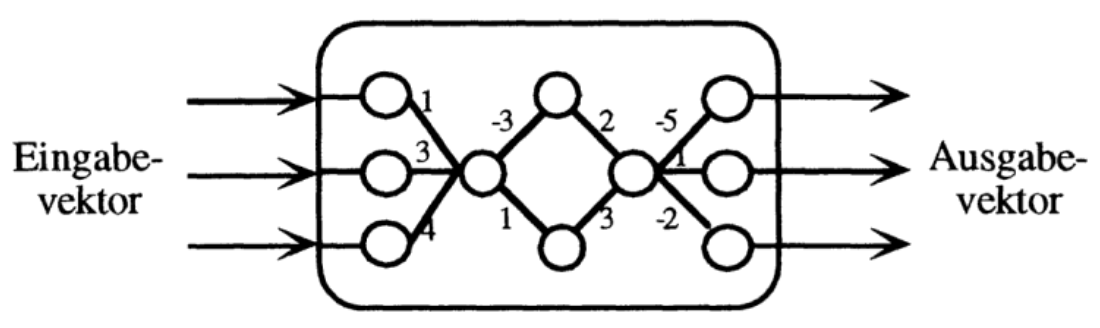
\includegraphics[width=0.50\textwidth]{knn}
    \caption{Schematische Darstellung eines Neuronalen Netzes}
    \label{Abb:basic}
    \end{figure}

\subsection{Merkmale}

\noindent \acp{KNN} zeichnen sich durch folgende Merkmale aus:

\begin{itemize}
    \item \acp{KNN} sind in der Lage, aus Beispielen zu lernen, ohne explizit programmiert zu werden. Dieser Vorgang wird als Lernen oder Training bezeichnet und ist der wichtigste Aspekt von \acp{KNN}. Das Lernen erfolgt durch Anpassung der Gewichtungen der Kanten zwischen den Neuronen, um die gewünschte Ausgabe zu erzeugen und wird wiederholt, bis die \ac{KI} bei bestimmten Eingaben das erwünschte Resultat erzeugt, oder zumindest annähert. Näheres dazu in Kapitel 2.
    \item \acp{KNN} sind sehr robust und fehlertolerant, da sie in der Lage sind, auch mit fehlerhaften oder unvollständigen Daten zu arbeiten. Dies ist ein großer Vorteil gegenüber herkömmlichen Algorithmen, die bei verrauschten Daten, wie sie beispielsweise in Sensormesswerten vorkommen, häufig nicht mehr zuverlässig funktionieren.
    \item \acp{KNN} können mit einer großen Menge an Daten umgehen und sind in der Lage, Muster in diesen Daten zu erkennen. Dadurch können Lernstrategien oder Entscheidungen auf Basis von Erfahrungen getroffen werden, was ideal für die Inter- und Extrapolation von Daten ist.
    \item \acp{KNN} bieten in ihrer Anwendungsphase eine durchaus gute Performanz, die sich mit der Größe des Netzes und der Anzahl der Trainingszyklen verbessert. Die Trainingsphase hingegen ist sehr rechenintensiv und kann je nach Größe des Netzes und der Anzahl der Trainingszyklen mehrere Stunden oder sogar Tage dauern. Zudem benötigt eine erfolgreiche Trainingsphase eine große Menge an qualitativen Trainingsdaten, die in der Regel manuell ausgewählt werden und vorsichtig administriert werden müssen.
    \end{itemize}
    

\newpage